%%%----------------------------------------------------------
\chapter{Circle detection in binary dot images}
\label{chap:ass01}
%%%----------------------------------------------------------

Humans can detect all kinds of shapes instinctively without even thinking about it while computers only \textit{see} a collection of pixels with certain values instead. Computer Vision tries to let computers see the same way humans do. Sometimes this can be achieved with more or less simple mathematical concepts and sometimes complex algorithms are required.

The task in the first assignment was to detect a circle which is embedded in a binary dot image. As humans we can easily recognize the circle and connect the points in our head but the computer does not know which image points actually belong to the circle. To detect the circle we are using a rather simple algorithm called RANSAC\cite{Ransac2020} created by Robert C.Bolles and Martin A.Fischer in the 1980s\cite{Fischler1981}.

\section{Algorithm}

To detect the circle the following steps were performed:
\begin{enumerate}
	\item Collect the coordinates of all points.
	\item Randomly choose 3 of them.
	\item Calculate the parameters ($x_c, y_c, r$)of a circle which passes through all 3 points.
	\item Count the points which are  on/close enough to the circle.
	\item Repeat the steps 2 to 4 a certain number of times and always  remember the circle with the most points on it.
	\item The "best-fitting" circle is the one which has the most points on it after a given number of iterations.
\end{enumerate}

\subsection{Collect all points}

All black pixels were saved as points with their respective x/y - coordinates into a collection by iterating over all the pixels of the image.

\subsection{Randomly choose 3 points}

3 points of that collection were randomly selected while making sure that no point was selected more than once.

\subsection{Calculate the circle parameters}

With the help of these 3 points it is possible to determine the attributes of a circle which passes through them as shown in Figure \ref{CalculateCircle} following an article from Paul Borke\cite{PaulBorke2020}.

\begin{figure}
	\centering
	\frame{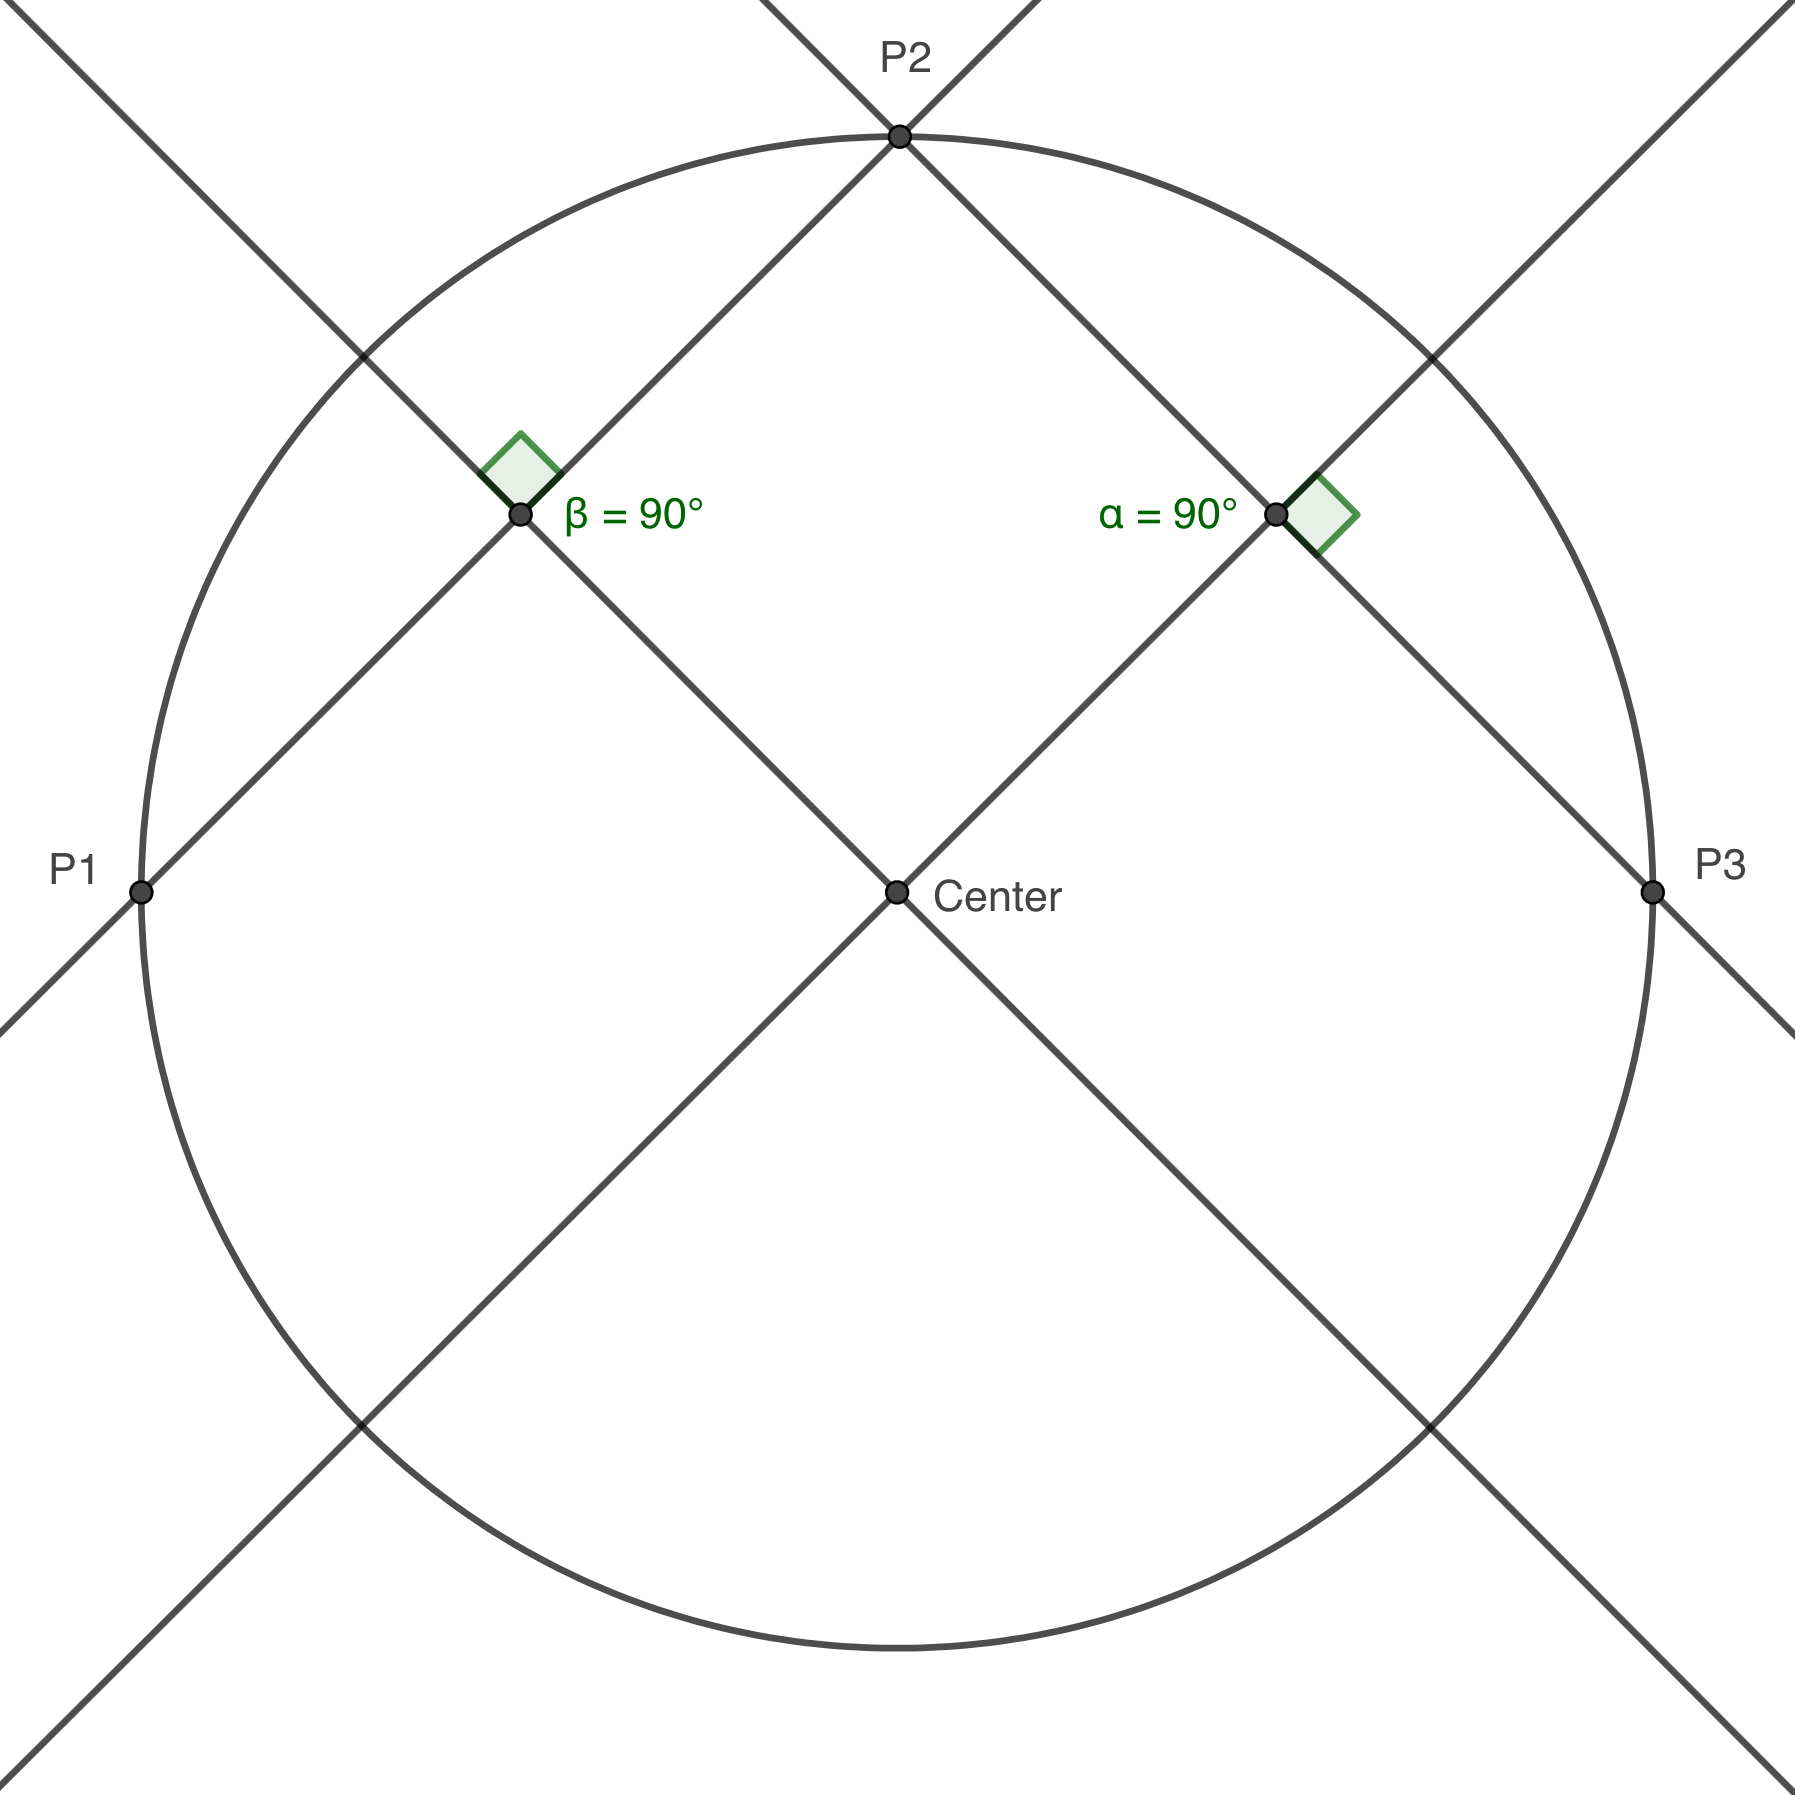
\includegraphics[width=.55\linewidth]{images/circlefrom3}}
	\caption{Determine the center of a circle with 3 points.}
	\label{CalculateCircle}
\end{figure}

A line through the point $P_1$ and $P_2$ was formed and another line through $P_2$ and $P_3$. The equations for these two lines are:
\begin{align*}
	y_a = m_a(x-x_1) + y_1\\
	y_b = m_b(x-x_2) + y_2
\end{align*}
These equations were rearranged to solve for their respective slopes $m$.
\begin{align}
	m_a& = \frac{y_2 - y_1}{x_2 - x_1}&
	m_b& = \frac{y_3 - y_2}{x_3 - x_2}
\end{align}
Now two lines perpendicular to the lines $y_a$($P_1P_2$) and $y_b$($P_2P_3$) going through the center between each point pair were created. The perpendicular of a line with a slope $m$ has a slope of $-1/m$. This results in following equations:
\begin{align}
	y'_a = -\frac{1}{m_a}(x-\frac{x_1 + x_2}{2}) + \frac{y_1 + y_2}{2}\label{perpendicular1}\\
	y'_b = -\frac{1}{m_b}(x-\frac{x_2 + x_3}{2}) + \frac{y_2 + y_3}{2}\label{perpendicular2}
\end{align}
The center of the circle is the intersection of these two perpendiculars. The x-value of the center was calculated with the following equation.
\begin{equation}
	x = \frac{m_am_b(y_1-y_3) + m_b(x_1+x_2) - m_a(x_2+x_3)}{2\cdot(m_b-m_a)}
\end{equation}
To calculate the y value of the center I substitute the x value into one of the two perpendiculars (\ref{perpendicular1}, \ref{perpendicular2}). The circle radius is determined by calculating the distance between the center point and one of the 3 originally chosen points.

There are 3 situations where a circle can not be calculated with just 3 points:
\begin{itemize}
	\item If all 3 points are collinear.
	\item If one of the 3 points was selected more than once. This gets checked while selecting the points.
	\item If one of the formed lines between 2 points is vertical the slope would be infinite. To avoid that the order of the 3 points is rearranged if this is the case. 
\end{itemize}

\subsection{Evaluate the circle}

After the circle's parameters were calculated the number of points on the circle got determined. The distance of all detected points to the center point of the circle and its difference to circle radius was calculated. If this difference is smaller than a given threshold, the point is considered on the circle. The threshold can be defined when the plugin is started. The number of points on the circle describes how well the circle "fits".

\subsection{Repeat}

This whole process gets repeated for a given number of times which can be defined at the start of the plugin. After each iteration the number of points on the calculated circle is compared to the number of points on the current "best-fitting" circle. If the count is higher the "best-fitting" circle gets replaced by the newly calculated circle. After this process reached the defined number of iterations the "best-fitting" circle was considered as the detected circle in the image.

\section{Results}
 
Figure \ref{BinaryInput} shows the generated test image. As soon as the described process was repeated for 25 times. The detected circle got drawn on the image in blue as well as all the points on it in red (Figure \ref{CircleResult}). It worked pretty well even on noisier images.

\begin{figure}
	\centering
	\begin{minipage}[t]{0.49\linewidth}
		\centering
		\frame{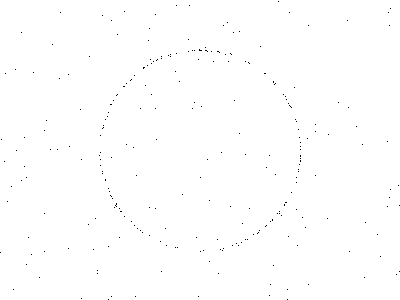
\includegraphics[width=.90\linewidth]{images/circle-test}}
		\caption{Generated noisy binary image.}
		\label{BinaryInput}
	\end{minipage}
	\hfill
	\begin{minipage}[t]{0.49\linewidth}
		\centering
		\frame{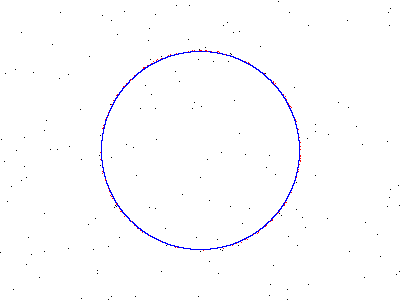
\includegraphics[width=.90\linewidth]{images/circle_result}}
		\caption{The Detected circle after 25 iterations and a threshold distance of 1 to the circle}
		\label{CircleResult}
	\end{minipage}
\end{figure}

\section{Research Questions}

\subsection{Question A}

\begin{itshape}
Assume n is the total number of points, of which m points belong to a circle.

\begin{itemize}
	\item What is the probability of selecting 3 circle points in a random draw?
	\item How many random draws are needed such that the probability of finding 3 circle
	points is 99\%
\end{itemize}
\end{itshape}

\vspace{3mm}

The probability of selecting one point which lies on the circle is: $\frac{m}{n}$. Now if 3 random points are chosen in a row the formula to calculate the probability is:
\begin{equation}
	P = \frac{m}{n} \cdot \frac{m-1}{n-1} \cdot \frac{m-2}{n-2}
	\label{probability}
\end{equation}
To calculate the number of random draws $n$ needed to select 3 circle points with a probability $W$ of 99\% we use following formula: $W = 1-(1-p)^n$ \cite{DanielaEder2020}. To calculate $p$ the formula above (\ref{probability}) is used then solve the equation (\ref{numberOfDraws}) to get the number of random draws $n$ needed that the probability of finding a circle is 99\%.
\begin{align}
	0.99& \geq 1 - (1-p)^n\\
	0.01& \geq (1-p)^n\\
	n& \geq \frac{\ln(0.01)}{\ln(1-p)}
	\label{numberOfDraws}
\end{align}

\subsection{Question B}

\textit{What if the image contains more than 1 circle and we want to find all of them? Develop (but do not implement)  a strategy for this case.}

\vspace{3mm}

To detect multiple circles in one image a threshold for the number of points which needed to be on a circle to be detected as a valid circle needs to be defined. If detected the circle is added to a list. To make sure that the same circle is not detected multiple times it has to be checked that there is no circle with the same center point and radius already in the list before adding it.